\subsubsection{V-Modell(e)}
\label{sec:Kap-2.2.1.2}

\sttpLeserfuehrung{Bilder/Kapitel-2/Leserfuehrung/Vorgehensmodelle-2-2-1-Illustration.pdf}{Bilder/Kapitel-2/Leserfuehrung/Vorgehensmodelle-2-2-1-2.pdf}

Wie beim Wasserfallmodell steckt hinter dem V-Modell eigentlich eine ganze Klasse von Modellen. Das ursprüngliche V-Modell aus den 1980er Jahren ist eine Erweiterung des Wasserfallmodells. Abbildung~\ref{fig:v-modell} zeigt ein V-Modell. 

%\sttpgls{Softwaretests}
%\sttpgls{Verifikation}
%\sttpgls{Validierung}

Wie das Wasserfallmodell gliedert das V-Modell den Softwareentwicklungsprozess in Phasen, die sequentiell ablaufen (linker Schenkel des V). Zusätzlich betont es aber explizit den hohen Stellenwert von Qualitätssicherungsmaßnahmen und stellt den Softwareentwicklungsprozessen daher Phasen mit Qualitätssicherungsprozessen gegenüber (rechter Schenkel).

\begin{figure}[h!]
	\centering
	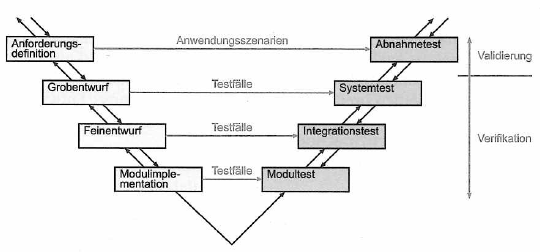
\includegraphics[scale=0.5]{Bilder/Kapitel-2/VModell.png}
	\caption{Ein V-Modell \cite[554]{bal08}}
	\label{fig:v-modell}
\end{figure}

Auf Grundlage des allgemeinen V-Modells wurde Ende der 1980er Jahre der V-Modell Entwicklungsstandard für IT-Projekte der Bundesrepublik Deutschland definiert – ursprünglich nur für Projekte des Verteidigungsministeriums, anschließend für alle Projekte der öffentlichen Hand in Deutschland. Das heute aktuelle und als geschützte Marke der Bundesrepublik Deutschland eingetragene V-Modell XT und seine Vorgänger legen und legten verbindliche Vorgehensweisen für Softwareentwicklungsprojekte des Bundes fest. Das V-Modell XT enthält sehr detaillierte Vorgaben zu Abläufen, Tätigkeiten und Ergebnissen der Phasen des Softwareentwicklungsprozesses und ist dementsprechend umfangreich. Da es sowohl für komplexe als auch für kleine Entwicklungsprojekte eingesetzt werden soll, sieht es vorzunehmende projektspezifische Anpassungen explizit vor. Einen solchen Anpassungsvorgang bezeichnet man als \textit{Tailoring}. \marginline{engl. to tailor sth. = etwas maßschneidern}
In der Regel erfolgt die Anpassung durch Reduktion von Arbeitspaketen des V-Modells XT – XT steht für Extreme Tailoring –, die für das konkrete Softwareentwicklungsprojekt nicht relevant sind. Im Gegensatz zu seinen Vorgängern, die rein sequentielle Modelle waren, soll das V-Modell XT auch die Einbettung agiler Methoden ermöglichen. Einen zusammenfassenden Überblick zum V-Modell XT geben \cite[620-637]{bal08} und \cite[105-110]{bro13}, ausführlich zum V-Modell XT \cite{hoe08} und zum Vorgänger V-Modell 97 \cite{dro00}. Zum allgemeinen V-Modell gibt \cite[553 \psqq]{bal08} einen Überblick. 